% This is part of Un soupçon de mathématique sans être agressif pour autant
% Copyright (c) 2012-2013
%   Laurent Claessens
% See the file fdl-1.3.txt for copying conditions.

% Ce fichier est celui pour les premières STMG.

\begin{center}

           \ifpdf
            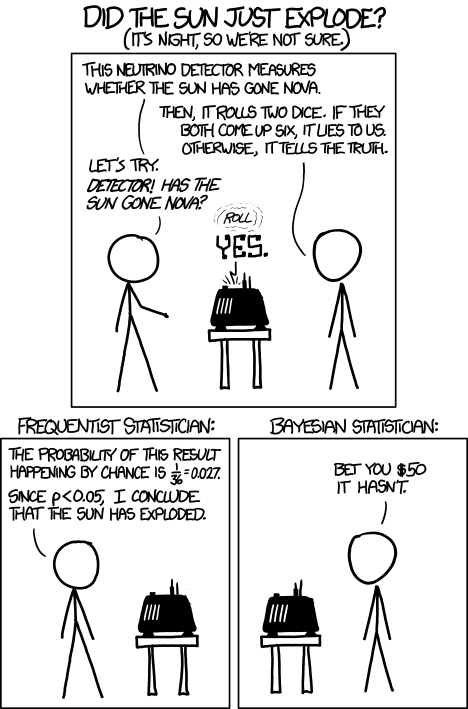
\includegraphics[width=8cm]{frequentists_vs_bayesians.png}
        \else
            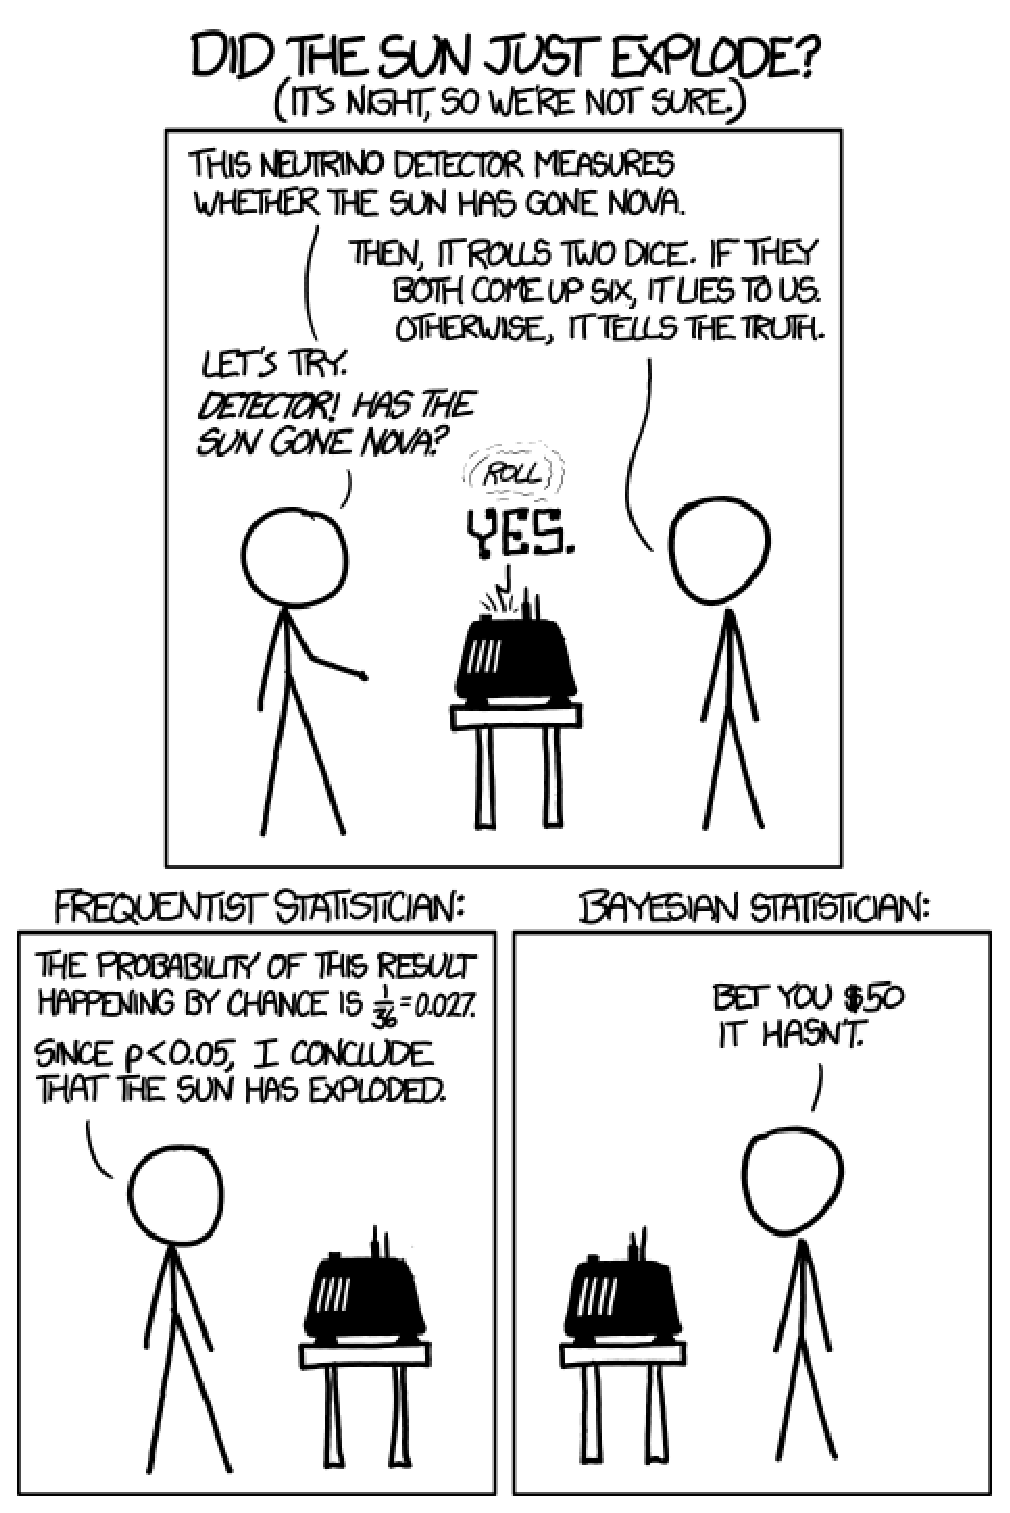
\includegraphics[width=8cm]{frequentists_vs_bayesians.eps}

            \fi

            \url{http://xkcd.com/1132/}, image publiée sous licence \href{http://xkcd.com/license.html}{CreativeCommons}.

\end{center}

Une chouette page concernant les intervalles de confiance à propos de l'élection à l'UMP est celle-ci :\\
\url{http://david.monniaux.free.fr/dotclear/index.php/post/2012/11/23/Le-sens-statistique-de-l-élection-à-l-UMP}

%+++++++++++++++++++++++++++++++++++++++++++++++++++++++++++++++++++++++++++++++++++++++++++++++++++++++++++++++++++++++++++ 
\section{Exercices}
%+++++++++++++++++++++++++++++++++++++++++++++++++++++++++++++++++++++++++++++++++++++++++++++++++++++++++++++++++++++++++++


\Exo{smath-0380}
\Exo{smath-0381}

